\section{Die Erd\H{o}s--Faber--Lov\'asz Vermutung}
Der Hauptteil dieser Bachelorarbeit befasst sich mit einer neuen Herangehensweise an die Erd\H{o}s--Faber--Lov\'asz Vermutung. Wir geben zuerst einen kurzen "Uberblick "uber die Vermutung und ihr Geschichte und behandeln dann Krauszzerlegungen von Graphen. 
\subsection{Die Geschichte der Vermutung}
Es bezeichne $\cE(n)$ die Klasse aller Graphen welche die Vereinigung von $n$ kantendisjunkten vollst"andigen Graphen der Ordnung $n$ sind. 
F"ur einen Graphen $G\in \cE(n)$ gibt es dann Graphen $G_1,G_2,\dots,G_n$ mit $G= \bigcup\limits_{i=1}^{n} G_i$, $G_i = K_n$ f"ur $1\leq i \leq n$ und $|G_i \cap G_j| \leq 1$ f"ur $1\leq i < j \leq n$. Dann ist $\omega(G) \geq n$ und somit gilt $\chi(G) \geq n$. Es ergibt sich dann die Frage, ob $G$ eine $n$-F"arbung besitzt.
\begin{figure}[h]
  \centering
  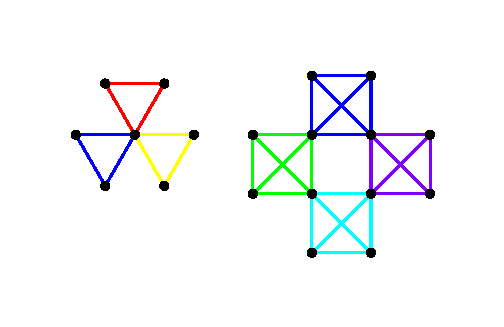
\includegraphics{images/bildeg3und4}
  \caption{Zwei Graphen aus $\cE(3)$ und $\cE(4)$}
  \label{fig:egraphen}
\end{figure}
\begin{conjecture}[Erd\H{o}s--Faber--Lov\'asz]
  F"ur jeden Graphen $G\in\cE(n)$ mit $n\in\N$ ist $\chi(G) \leq n$.
  \label{con:efl}
\end{conjecture}
Die Vermutung wurde 1972 in Ohio von Erd\H{o}s, Faber und Lov\'asz aufgestellt, als sie "uber eine Verallgemeinerung der Vizing-Schranke f"ur lineare Hypergraphen nachdachten (siehe \cite{FaberL74} und \cite{Erdos76}). Bereits sieben Jahre sp"ater bot Erd\H{o}s schon 500 Dollar f"ur die L"osung des Problems \cite{Erdos79j}.
Diese Vermutung geh"orte zu Erd\H{o}s drei Lieblingsproblemen (siehe \cite{Erdos81}).

Vermutung \ref{con:efl} ist "aquivalent zu der folgenden Vermutung "uber lineare Hypergraphen (siehe Satz \ref{thm:equivefl}):
\begin{conjecture}[Erd\H{o}s--Faber--Lov\'asz]
  F"ur jeden linearen Hypergraphen $H$ ist $\chi'(H) \leq |H|$.
  \label{con:eflhyper}
\end{conjecture}

Im Folgenden wollen wir einige Resultate zur Vermutung \ref{con:efl} anf"uhren. Chung und Lawler \cite{ChungL88} bewiesen die folgende obere Schranke f"ur die chromatische Zahl von Graphen aus $\cE(n)$:

\begin{theorem}
  F"ur jeden Graphen $G\in\cE(n)$ mit $n\in\N$ ist $\chi(G) \leq \frac{3n}{2}-2$.
  \label{thm:ChungLawler}
\end{theorem}
Kahn \cite{Kahn92} verbesserte diese obere Schranke, indem er bewies, dass die Vermutung asymptotisch wahr ist.
\begin{theorem}
  F"ur jeden linearen Hypergraphen $H$ ist $\chi'(H) \leq |H| + o(|H|)$.
  \label{thm:kahn}
\end{theorem}

Es ist au{\ss}erdem bekannt, das Vermutung \ref{con:efl} f"ur $n\leq 10$ gilt, wie Hindman \cite{Hindman81} bewies.
Weitere Anmerkungen und Resultate finden sich in \cite{RomeroS2007}.

\subsection{Krauszzerlegungen von Graphen}
Die Graphen aus $\cE(n)$ lassen sich alle durch $n$ vollst"andige Graphen der Ordnung $n$ kantendisjunkt "uberdecken. Im Folgenden wollen wir ein allgemeineres Konzept betrachten, indem wir nicht fordern, dass alle Graphen der "Uberdeckung dieselbe Ordnung haben. 
Diese Art der "Uberdeckung wurde zuerst von Krausz \cite{Krausz43} zur Charakterisierung von Kantengraphen verwendet, daher der Name Krauszzerlegung. 

Sei $G$ ein Graph und $\mathcal{K}$ eine Menge Untergraphen von $G$. Man nennt $\mathcal{K}$ dann eine Krauszzerlegung von $G$, falls folgende Bedingungen erf"ullt sind:
\begin{enumerate}
  \item[\rm{(K1)}] Jeder Graphen $K\in \mathcal{K}$ ist ein vollst"andiger Graph der Ordnung $|K| \geq 2$. 
  \item[\rm{(K2)}] Sind $K,K'\in \mathcal{K}$ unterschiedlich, so sind sie kantendisjunkt (d.h. $|K\cap K'| \leq 1$).
  \item[\rm{(K3)}] $\mathcal K$ ist eine "Uberdeckung von $G$, d.h.  $G=\bigcup\limits_{K\in \mathcal K}K$.
\end{enumerate}
Desweiteren sei f"ur $v\in V(G)$ der \DF{Grad} von $v$ bez"uglich $\mathcal K$ definiert als $$d_{\mathcal{K}}(v) = |\{ K\in\mathcal K \;|\;  v \in V(K)\}|.$$ Der \DF{Minimalgrad} von $\mathcal K$ ist $$\delta(\mathcal K) = \min\limits_{v\in V(G)}d_{\mathcal{K}}(v)$$ und der \DF{Maximalgrad} von $\mathcal{K}$ ist $$\Delta(\mathcal{K}) = \max\limits_{v\in V(G)}d_{\mathcal{K}}(v).$$

Krausz \cite{Krausz43} besch"aftigte sich mit der Frage, welche Graphen Kantengraphen von Graphen sind. Er bewie{\ss}, dass ein Graph genau dann ein Kantengraph eines Graphen ist, wenn es eine Krauszzerlegung mit Maximalgrad h"ochstens $2$ besitzt. Ist $G=L(H)$ der Kantengraph des Graphen $H$, so ist f"ur jede Ecke $v\in V(H)$ die Kantenmenge $E_H(v)$ eine Clique von $G$ und somit ist $K^{v}=G[E_H(v)]$ ein vollst"andiger Graph. F"ur zwei verschiedene Ecken $u,v\in V(H)$ gilt dann:
$$K^{u}\cap K^{v} \neq \varnothing \Leftrightarrow uv \in E(H) \Leftrightarrow |K^{u} \cap K^{v}| \leq 1.$$
Sind nun $e,e'\in E(H)$ zwei adjazente Kanten von $H$ und somit $ee'$ eine Kante von $G$, so gibt es eine Ecke $v\in e\cap e'$ und $e,e'$ geh"oren zu $K^{v}$. Also ist $\mathcal{K} = \set{K^{v}}{v\in V(H)}$ eine Krauszzerlegung von $G$ mit $\Delta(\mathcal{K}) \leq 2$.

F"ur $d \geq 1$ sei $\kappa_d(G)$ die kleinste positive Zahl $m$ derart, dass $G$ eine Krauszzerlegung $\mathcal K$ mit $|\mathcal K| = m$ und $\delta(\mathcal K) \geq d$ besitzt. Existiert keine solche Zahl $m$, so setzen wir $\kappa_{d}(G) = \infty$.

\begin{figure}[htb]
  \centering
  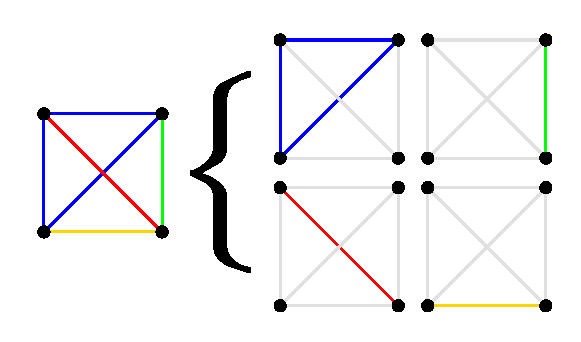
\includegraphics{images/k4decomp.eps}
  \caption{Eine Krauszzerlegung des $K_4$}
  \label{fig:KrauszzerlegungK4}
\end{figure}
In Abbildung \ref{fig:KrauszzerlegungK4} sehen wir eine Krauszzerlegung $\mathcal{K}$ des $K_4$ (die einzelnen kantendisjunkten Untergraphen sind jeweils mit der selben Farbe markiert). Wir k"onnen au{\ss}erdem erkennen, dass $\delta(\mathcal{K}) = 2$ und folglich $\kappa_{2}(K_4) \leq 4$ (wir werden sp"ater sehen, dass stets $\kappa_{2}(K_n) \geq n$ gilt und somit $\kappa_{2}(K_{4}) = 4$ ist). 

\begin{figure}[htb]
  \centering
  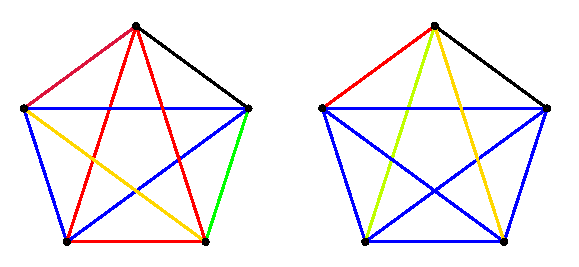
\includegraphics{images/K5krauszdecomp.eps}
  \caption{Zwei Krauszzerlegungen des $K_5$}
  \label{fig:KrauszzerlegungK5}
\end{figure}

In Abbildung \ref{fig:KrauszzerlegungK5} sehen wir zwei Krauszzerlegungen des $K_5$, beide mit Minimalgrad $2$. 

\begin{lemma}
  Seien $G$ ein Graph und $d\in \N$. Genau dann ist $\kappa_{d}(G) < \infty$, wenn $\delta(G) \geq d$ ist. 
  \label{lm:krauszexistenz}
\end{lemma}

\begin{proof}
  Wir zeigen zun"achst, dass $\delta(G) \geq d$ ist, falls $p = \kappa_d(G) < \infty$. Sei $v\in V(G)$ mit $d_{G}(v) = \delta(G)$. Dann existiert eine Krauszzerlegung $\mathcal{K}=\left\{ K^{1}, \dots , K^{p} \right\}$ von $G$ mit $\delta(\mathcal{K}) \geq d$. Da alle Graphen der Krauszzerlegung kantendisjunkt sind, gilt $$ d \leq \sum\limits_{K\in \mathcal{K}, v\in K} d_{K}(v) \leq d_{G}(v) = \delta(v).$$
  Dabei gilt die erste Ungleichung, da $v$ in mindestens $d$ der Graphen aus $\mathcal{K}$ vorkommt und in diesen mindestens Grad $1$ hat.

  Sei nun $\delta(G) \geq d$. Wir m"ussen zeigen, dass es eine Krauszzerlegung $\mathcal{K}$ mit
  $d_{\mathcal{K}}(v) \geq d$ f"ur alle $v\in V(G)$ gibt. Sei $E(G)= \{e_1,\dots, e_{m}\}$ eine Nummerierung der Kanten. Sei dann $K^i$ der Graph, welcher nur aus der Kante $e_i$ und den zu $e_i$ inzidenten Kanten besteht. Wir zeigen: $\mathcal{K} = \left\{ K^i \;|\; 1 \leq i \leq m \right\}$ ist eine Krauszzerlegung von $G$ mit $\delta(\mathcal{K}) \geq d$. (K1) ist erf"ullt, da alle Graphen von $\mathcal{K}$ isomorph zu $K_{2}$ sind. Sind $K,K'$ zwei verschiedene Graphen aus $\mathcal{K}$, so sind sie
  kantendisjunkt, da ihre einzigen Kanten in $G$ verschieden sind. Also ist auch (K2) erf"ullt. Da jede Kante von $G$ in einem $K\in \mathcal{K}$ vorkommt, ist auch (K3) erf"ullt. Sei nun $v$ eine Ecke von $G$. Dann ist $$d_{\mathcal{K}}(v) = d_{G}(v) \geq \delta(G) \geq d$$ und folglich auch $\delta(\mathcal{K}) \geq d$. Damit ist gezeigt, dass $\mathcal{K}$ eine Krauszzerlegung von $G$ ist mit $\delta\left( \mathcal{K} \right) \geq d$. Also ist
  $\kappa_{d}(G) \leq |\mathcal{K}| <
  \infty$.
\end{proof}

\begin{example}
  Sei $G$ ein dreiecksfreier Graph mit Minimalgrad mindestens $d$. Dann ist $\kappa_{d}(G) = |E(G)|$, da $G$ keine Dreiecke enth"alt und somit jeder Graph einer Krauszzerlegung von $G$ isomorph zu $K_{2}$ sein muss. 
\end{example}

Wir werden nun einen Zusammenhang zwischen Krauszzerlegungen und der Erd\H{o}s--Faber--Lov\'asz Vermutung herstellen.

\begin{theorem}
  Die folgenden Aussagen sind "aquivalent:
  \begin{enumerate}[label=\rm{(\alph*)}]
    \item F"ur alle $n\in\N$ und alle $G\in\cE(n)$ gilt $\chi(G) \leq n$.
    \item F"ur alle linearen Hypergraphen $H$ gilt $\chi'(H) \leq |H|$.
    \item F"ur alle Graphen $G$ gilt $\chi(G) \leq \kappa_{2}(G)$.
  \end{enumerate}
  \label{thm:equivefl}
\end{theorem}

\begin{proof}
  Wir zeigen zuerst, dass (b) aus (a) folgt. Sei dazu $H$ ein linearer Hypergraph der Ordnung $n$ und $G=L(H)$ sein Kantengraph. Sei $v\in V(H)$ eine Ecke von $H$. Wir betrachten dann $K^{v} = G[E_H(v)]$. Dann ist $K^{v}$ ein vollst"andiger Graph. Wir zeigen, dass seine Ordnung h"ochstens $n-1$ ist. Angenommen, das ist nicht der Fall. 
\begin{figure}[h]
  \centering
  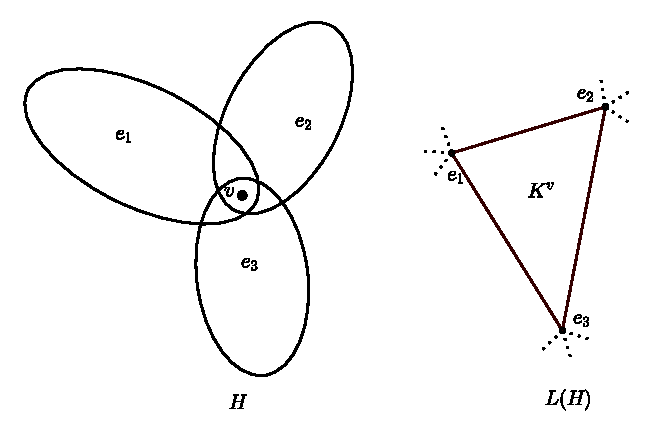
\includegraphics{images/KvLinegraph.eps}
  \caption{Die Beziehung von $v$ und $K^{v}$}
  \label{fig:kvlinegraph}
\end{figure}
  Dann ist die Ordnung von $K^{v}$ mindestens $n$ und wir finden $n$ unterschiedlich Kanten in $E_H(v)$, welche $v$ enthalten. 
  Da $H$ ein linearer Hypergraph ist, ist $v$ die einzige Ecke die zwei Kanten aus $E_{H}(v)$ gemeinsam haben, d.h. $|e\cap e'| = |\{ v \}| = 1$ f"ur alle $\{e,e'\} \in [E_H(v)]^{2}$. Au{\ss}erdem ist $|e| \geq 2$ f"ur alle $e\in E(H)$. 
  Dann folgt aber, dass $$|H| \geq |\bigcup\limits_{e\in E_H(v)} e| = \sum\limits_{e\in E_{H}(v)} |e\setminus \{v\}|+ | \{v\}| \geq n+1$$ gilt, ein Widerspruch zur Voraussetzung $|H| = n$. 
  Also ist $K^{v}$ ein vollst"andiger Graph der Ordnung h"ochstens $n-1$. Wir bezeichnen dann mit $\tilde{K^{v}}$ den vollst"andigen Graphen der Ordnung $n$, der aus $K^{v}$ entsteht indem wir die n"otige Anzahl Ecken und Kanten hinzuf"ugen. 
  Es bezeichne dann $\tilde{G}$ den Graphen, den wir aus $G$ erhalten, indem wir alle Ecken und Kanten die wir so hinzugef"ugt haben auch zu $G$ hinzuf"ugen. 
  Dann ist $G$ ein induzierter Untergraph von $\tilde{G}$. 
  Wir zeigen jetzt, dass $\mathcal{K}= \set{K^{v}}{v\in V(H)}$ eine Krauszzerlegung von $G$ ist. 
  (K1) ist trivialerweise erf"ullt. Um (K2) zu zeigen, nehmen wir an das in $G$ eine Kante $ee'\in E(G)$ exisitert, welche in zwei verschiedenen Graphen $K,K'$ von $\mathcal{K}$ vorkommt.
  Dann existieren zwei unterschiedliche Ecken $u,v$ von $H$ f"ur welche $K= K^{v}$ und $K' = K^{w}$ gilt. 
  Da $e,e'\in V(K^{v}) \cap V(K^{w})$ gilt, kommen die Ecken $v$ und $u$ von $H$ also sowohl in $e$ als auch in $e'$ vor. Damit ist $|e\cap e'| \geq 2$, ein Widerspruch zur Voraussetzung, dass $H$ ein linearer Hypergraph ist. Damit gilt (K2).
  Sei $ee'\in V(G)$ eine Kante von $G$. Da $G$ der Kantengraph von $H$ ist, existiert eine Ecke $v\in V(H)$ mit $ v\in e\cap e'$. 
  Also ist $ee'\in K^{v}\in \mathcal{K}$. Damit ist auch (K3) gezeigt. Also ist $\mathcal{K}$ eine Krauszzerlegung von $G$. Insbesondere ist auch $\tilde{\mathcal{K}} = \set{\tilde{K^{v}}}{v\in V(H)}$ eine Krauszzerlegung von $\tilde{G}$. Also ist $\tilde{G}\in \cE(n)$. Mit (a) folgt dann $$ \chi'(H) = \chi(G) \leq \chi(\tilde{G}) \leq n = |H|.$$
  
Als n"achstes zeigen wir, dass (c) aus (b) folgt. 
  Dazu betrachten wir einen beliebigen Graphen $G$ und zeigen, dass $\chi(G) \leq \kappa_{2}(G)$ gilt. Ist $\kappa_{2}(G) = \infty$, so ist nichts zu zeigen. Andernfalls ist $\kappa_{2}(G) = p < \infty $ und es gibt eine Krauszzerlegung $\mathcal{K}= \left\{ K^{1},\dots,K^{p} \right\}$ von $G$ mit $\delta(\mathcal{K}) \geq 2 $.  
  \todo{bild von hypergraph konstruktion}
  F"ur $v\in V(G)$ definieren wir $e_v$ als die Menge aller $K\in \mathcal{K}$, welche $v$ enthalten. Da $\mathcal{K}$ eine Krauszzerlegung ist, gilt $|e_v| = d_{\mathcal{K}}(v)\geq \delta(\mathcal{K}) \geq 2$ f"ur alle $v \in V(G)$. Sei $H$ der Hypergraph mit Eckenmenge $\mathcal{K}$ und Kantenmenge $\left\{ e_v\;|\; v\in V(G) \right\}$. Wir betrachten $\pi: V(G) \mapsto E(H)$ mit $\pi(v) = e_v$, diese ist offensichtlich surjektiv. Wir zeigen, dass $\pi$ bijektiv ist. W"are dem nicht so, so g"abe es zwei unterschiedliche Ecken $v,w$ mit $e_v = e_w$. 
  Da $|e_v| \geq 2$ ist,  w"are dann die Kante $vw$ in zwei Graphen von $\mathcal{K}$ enthalten, was der Bedingung (K2) widerspr"ache. Also ist $\pi$ bijektiv.
  Wir zeigen nun, dass $H$ ein linear Hypergraph ist. 
  Seien dazu $e_{v},e_{w} $ zwei unterschiedliche Kanten von $H$.
  Angenommen $|e_{v}\cap e_{w}| \geq 2$. Dann existieren mindestens zwei Graphen $K,K' \in \mathcal{K}$ mit $v,w \in K,K'$. Da $K,K'$ aus der Krauszerlegung sind, ist die Kante $vw$ sowohl in $K$ als auch in $K'$ vorhanden. Dies ist aber ein Widerspruch zu Eigenschaft (K2) einer Krauszzerlegung.
  Folglich ist $|e_{v}\cap e_{w}| \leq 1$, also ist $H$ linear. Dann folgt aus der Vorraussetzung (b), dass $\chi'(H) \leq |H| = \kappa_{2}(G)$ ist.
  Somit finden wir eine F"arbung $\phi : E(H) \mapsto \left\{ 1,\dots,p \right\}$ der Kanten von $H$. Sei dann $\varphi =  \phi \circ \pi$. Wir zeigen, dass $\varphi$ eine F"arbung der Ecken von $G$ ist. Dazu betrachten wir eine Kante $vw\in E(G)$. Dann existiert ein $K\in \mathcal{K}$ mit $vw\in E(K)$. Also ist $e_v\cap e_w \neq \varnothing$ und folglich \begin{equation*}
    \varphi(v) = \phi(e_v) \neq \phi(e_w) = \varphi(w).
  \end{equation*} 
  Also ist $\varphi$ ein $p$-F"arbung von $G$. Das hei{\ss}t
  \begin{equation*}
    \chi(G) \leq p = \kappa_{2}(G).
  \end{equation*}
  Also folgt (c) aus (b).

  Nun zeigen wir, dass (a) aus (c) folgt. 
  Sei $G\in \cE(p) $ mit $p\in \N$. Dann ist $G$ die kantendisjunkte Vereinigung von $p$ vollst"andigen Graphen der Ordnung $p$, welche wir mit $K^{1},\dots, K^{p}$ bezeichnen wollen. Nun entfernen wir wiederholt Ecken aus $G$,  deren aktueller Grad kleiner als $p$ ist solange, bis keine Ecken vom Grad kleiner als $p$ existieren. Den daraus resultierenden (m"oglicherweise leeren) Graphen nennen wir $H$. 
  Gelingt es, $H$ mit $p$ Farben zu f"arben, so k"onnen wir diese F"arbung schrittweise zu einer F"arbung von $G$ erweitern, indem wir die entfernten Ecken in umgekehrter Reihenfolge f"arben. Dies ist mit $p$ Farben m"oglich, da jede zu f"arbende Ecke h"ochstens $p-1$ bereits gef"arbte Nachbarn besitzt.
  Somit reicht es zu zeigen, dass $\chi(H) \leq p$ ist. Ist $V(H) =\varnothing$, so gilt dies trivialerweise. Andernfalls gilt nach Konstruktion $\delta(H) \geq p $. 
  Sei $\hat{K}^i = K^{i} \cap H$ f"ur $1\leq i \leq n$. Dann ist $\hat{K}^i$ ein vollst"andiger Graph f"ur alle $i$. W"ahle $\mathcal{K} = \left\{ \hat{K}^i \;|\; | \hat{K}^i| \geq 2  , 1\leq i \leq n\right\}$. Wir zeigen, dass $\mathcal{K}$ eine Krauszzerlegung von $H$ mit $\delta(\mathcal{K}) \geq 2$ ist.
  Die Bedingung (K1) ist offensichtlich erf"ullt. Da in $G$ die $K^{i}$ kantendisjunkt sind und $H$ ein induzierter Untergraph von $G$ ist sind die $\hat{K}^{i}$ in $H$ ebenfalls kantendisjunkt. Folglich ist die Bedingung (K2) ebenfalls erf"ullt. Sei $v\in V(H)$. Dann ist $d_{H}(v) \geq p$ und somit gilt $d_{G}(v) \geq d_H(v) \geq p$. 
  Die Ecke $v$ ist in mindestens zwei vollst"andigen Graphen $K$ und $K'$ aus der Krauszzerlegung $\mathcal{K}$ enthalten. 
  Ansonsten w"are $v$ nur in einem vollst"andigen Graphen $K \in \mathcal{K}$ enthalten und somit w"are $d_{H}(v) = d_{K}(v) \leq p-1$, was unm"oglich ist. 
  Folglich ist $d_{\mathcal{K}}(v) \geq 2$ f"ur alle $v \in V(H)$. Also ist $\mathcal{K}$ eine Krauszzerlegung mit $\delta(\mathcal{K}) \geq 2$ und wegen (c) folgt dann:
  \begin{equation*}
    \chi(H) \leq \kappa_{2}(H) \leq |\mathcal{K}| \leq p .
  \end{equation*}
  Also l"asst sich $H$ mit $p$ Farben f"arben und wir k"onnen wie oben beschrieben $G$ ebenfalls mit $p$ Farben f"arben. Also ist $\chi(G) \leq p$.
\end{proof}

Aus dem vorhergehenden Satz folgt, dass Vermutung \ref{con:efl} und Vermutung \ref{con:eflhyper} "aquivalent sind. Eine weitere dazu "aquivalente Vermutung ist die folgende:

\begin{conjecture}
  F"ur jeden Graphen $G$ ist $\chi(G) \leq \kappa_{2}(G)$. 
  \label{con:eflkrausz}
\end{conjecture}

Im Zusammenhang mit diesen Vermutungen ist es sinnvoll, die folgenden Extremalfunktionen zu betrachten:
\begin{align*}
  f_1(n) &= \max \set{\chi(G)}{G\in \bigcup \limits_{p=1}^{n} \cE(p)} \\
  f_2(n) &=  \max \set{\chi'(H)}{H \text{ ist ein linearer Hypergraph mit } |H| \leq n} \\
  f_3(n) &= \max \set{\chi(G)}{G \text{ ist ein Graph mit }\kappa_{2}(G) \leq n}
\end{align*}
f"ur $n \geq 3$. 
Der Beweis von Satz \ref{thm:equivefl} l"asst sich dann ohne Schwierigkeiten modifizieren, dass man zeigen kann $$f_1(n) = f_2(n) = f_3(n) $$ f"ur alle $n\geq 3$. 

